\documentclass[9pt]{beamer}

%\usepackage{tikz}
\usepackage{amsmath}
\usepackage{amsfonts}
\usepackage{amssymb}
\usepackage{algorithm2e}
\usepackage{color, colortbl}
\usepackage{enumerate}
\usepackage{arydshln}
\usepackage{multirow}

\usepackage{animate}
\usepackage{tabularx}

\renewcommand{\figurename}{Fig}
\usetheme{uha}



%\theoremstyle{plain}
%  \newtheorem{theorem}{Theorem}
%  \newtheorem{lemma}{Lemma}
\newtheorem{corrolary}{Corollary}
\newtheorem{claim}{Claim}
\newtheorem{proposition}{Proposition}
\newtheorem{property}{Property}
%  \newtheorem{fact}{Fact}
%\theoremstyle{definition}
%  \newtheorem{definition}{Definition}
%  \newtheorem{example}{Example}
%\theoremstyle{remark}
\newtheorem{remark}{Remark}
\newtheorem{proviso}{Proviso}


\newcommand{\ccr}[1]{{\color{red}#1}}
\newcommand{\ccb}[1]{{\color{blue}#1}}
\newcommand{\ccp}[1]{{\color{purple}#1}}
\newcommand{\ccm}[1]{{\color{magenta}#1}}
\newcommand{\cco}[1]{{\color{orange}#1}}
\newcommand{\ccy}[1]{{\color{yellow}#1}}
\newcommand{\ccl}[1]{{\color{lime}#1}}
\newcommand{\ccc}[1]{{\color{cyan}#1}}
\newcommand{\ccg}[1]{{\color{gray}#1}}
\newcommand{\ccpk}[1]{{\color{pink}#1}}
\newcommand{\ccov}[1]{{\color{olive}#1}}


\begin{document}

%%//////////////////////////////////////////////////////////////////////////////////////////////%%1

\title{Community Detection}
\subtitle{Algorithm Design}
\author{Zhemin Huang, Xunjie Wang}
\institute{School of Software, Shanghai Jiao Tong University}
\date{\hspace{2em}}
\frame{
	\titlepage
}

%%//////////////////////////////////////////////////////////////////////////////////////////////%%1

\section{Problem Description}

\frame{
	\frametitle{Network}
	\begin{definition}
		[Network]
		A \ccp{network} is represented as \ccb{$G=(V,E,W)$},\\
		where \ccb{$V,E$} denote the set of nodes and edges, respectively, and \ccb{$W$} denotes the corresponding weights of the connections.
	\end{definition}

	\bigskip

	\centerline{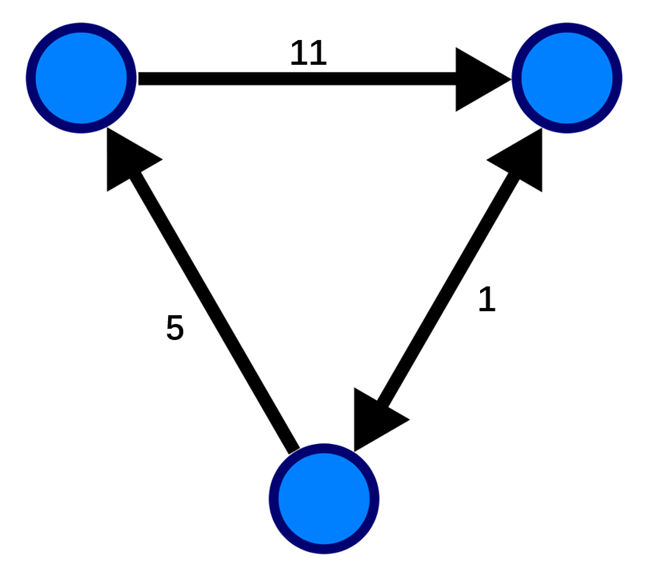
\includegraphics[width=0.4\textwidth]{figures/network/network.png}}
}

\frame{
	\frametitle{Community}
	\begin{definition}
		[Community]
		Communities are the sub-graphs in a network, where nodes share dense connections. Sparsely-connected nodes cripple communities. \\
		We use \ccb{$C=\{C_1,C_2,...,C_k\}$} to denote a set of \ccb{$k$} communities divided from a network \ccb{$G$}. A node \ccb{$v$} clustered into the community \ccb{$C_i$} satisfies the condition that the internal degree of each node inside the community exceeds its external degree. \\
		For \ccb{$\forall i,j, C_i\in C, C_j\in C$}, they satisfy the following conditions
		\ccb{
			\begin{equation*}
				C_i\cap C_j=\varnothing
			\end{equation*}
			\begin{equation*}
				\bigcup_{i=1}^{k}C_i=G
			\end{equation*}
		}
	\end{definition}
}

\frame{
	\frametitle{Community}
	A community is a type of sub-graph that represents some real social phenomenon. In order words, a community is a group of people or objects, which \ccp{share common characteristics}.

	\centerline{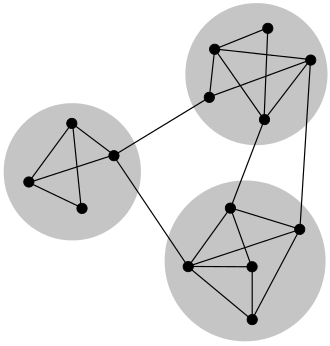
\includegraphics[width=0.5\textwidth]{figures/network/community.png}}
}

\frame{
	\frametitle{Modularity}
	\begin{definition}
		[Modularity]
		Consider a particular division of a network into \ccb{$k$} communities. Let us define a \ccb{$k \times k$} symmetric matrix \ccb{$e$} whose element \ccb{$e_{ij}$} is the fraction of all edges in the network that link vertices in community \ccb{$i$} to vertices in community \ccb{$j$}.\\
		We further define the row sums \ccb{$a_i=\sum_{j}e_{ij}$}, which represent the fraction of edges that connect to vertices in community \ccb{$i$}.\\
		In a network in which edges fall between vertices who belong to different communities, we would have \ccb{$e_{ij}=a_ia_j$}. Let \ccb{$||X||$} indicates the sum of the elements of the matrix \ccb{$X$}.
		Thus, we define modularity by
		\ccb{
			\begin{equation*}
				Q=\sum_i{e_{ii}-{a_i}^2}=\sum_i{e_{ii}}-\sum_i{{a_i}^2}=Trace-||e^2||
			\end{equation*}
		}
	\end{definition}
}

\frame{
	\frametitle{Modularity}
	Proposed by Mark Newman, UMich.
	
	\noindent He is known for his fundamental contributions to the fields of complex networks and complex systems, for which he was awarded the 2014 Lagrange Prize.
	\vspace{1cm}	
	\href{http://www-personal.umich.edu/~mejn/}{
		\centerline{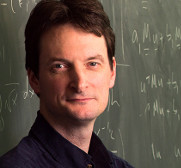
\includegraphics[width=0.45\textwidth]{figures/gn/newman.jpg}}
	}
}

\frame{
	\frametitle{Modularity}
	Modularity was designed to measure the strength of division of a network into communities. 
	
	\noindent If \ccb{$Q$} is high, we get strong community structure.
	
	\noindent In practice, values for such networks typically fall in the range from about \ccb{0.3} to \ccb{0.7}.
	\centerline{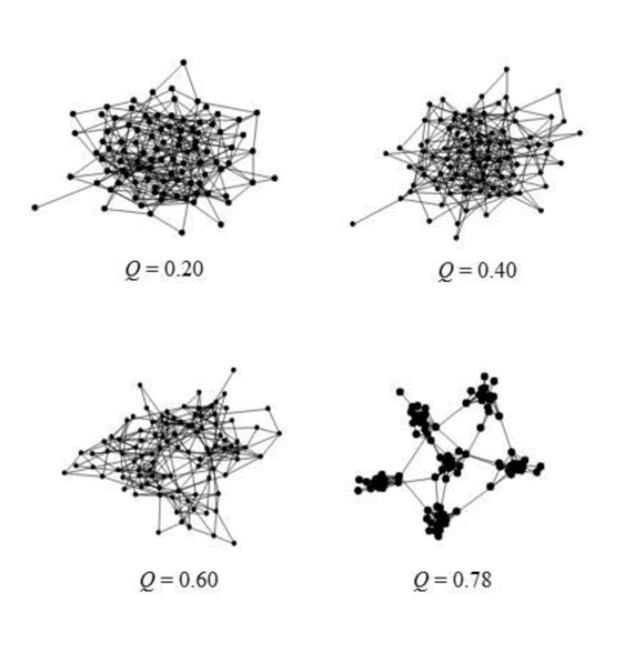
\includegraphics[width=0.5\textwidth]{figures/network/modularity.png}}
}

\frame{
	\frametitle{Reformulation of The Modularity}
	In order to raise \ccp{a spectral algorithm for community detection}, Newman redefined the concept of modularity.
	\begin{definition}
		[Reformulation of The Modularity]
		The modularity of a community partition is a scalar ranging from \ccb{$-\frac{1}{2}$} to \ccb{$1$} that evaluates the density of links inside communities as compared to links between communities. \\
		For a given graph \ccb{$G$}. Let \ccb{$A_{ij}$} be the weight of the edge between \ccb{$i$} and \ccb{$j$}, \ccb{$k_{i}=\sum_{(i, j) \in E}A_{ij}$} is the sum of the weights of all the edges attached to vertex \ccb{$i$},  \ccb{$m = \frac{1}{2}\sum_{ij}A_{ij}$}, the quantity \ccb{$\frac{1}{2}(s_is_j+1)$} is \ccb{1} if \ccb{$i$} and \ccb{$j$} are in the same group and \ccb{0} otherwise, \\
		\ccb{
			\begin{equation*}
				Q = \frac{1}{4m}\sum_{i \in V, j \in V}(A_{ij} - \frac{k_{i}k_{j}}{2m})\frac{1}{2}(s_is_j+1)
			\end{equation*}}
	\end{definition}
	The leading factor of \ccb{$\frac{1}{4m}$} seems to be confusing. Actually, it is included for compatibility with the previous definition of modularity.
}

\frame{
	\frametitle{Community Detection}
	From the definitions above, we can lead to our goal -- \ccp{community detection}.
	\begin{definition}
		[Community detection]
		Community detection is a method to extract communities from large networks when the modularity is optimal.
	\end{definition}
	Not all methods are based on modularity, such as \ccp{Infomap}.
	
	\noindent Modularity has its limits, but it is still the most commonly used method for evaluating results.
}

\section{Key Properties}

\frame{
	\frametitle{Modularity}
	\begin{lemma}
		We denote the set of all possible communities of a graph \ccb{$G$} with \ccb{$A(G)$}, \ccb{$Q(P)$} refers to the modularity of \ccb{$P$}. \\
		Let \ccb{$G$} be an undirected and unweighted graph and \ccb{$P \in A(G)$}. \\
		Then \ccb{$-\frac{1}{2}\le Q(P) \le 1$} holds.
	\end{lemma}
}

\frame{
	\frametitle{Proof}
	\ccm{\em Proof.}
	Let \ccb{$m_i=|E(P)|$} be the number of edges inside community \ccb{$P$} and \ccb{$m_e=\sum_{P\neq P'\in P}|E(P, P')|$} be the number of edges having exactly one end-node in \ccb{$P$}. \\
	Then we can calculate the contribution of \ccb{$P$} to \ccb{$Q(P)$}
	\ccb{
		\begin{equation*}
			\frac{m_i}{m}-(\frac{m_i}{m}+\frac{m_e}{2m})^2=\frac{-4(m_i)^2+4m_i(m-m_e)-(m_e)^2}{4m^2}
		\end{equation*}
	}

	It is obvious that the only maximum point is at \ccb{$m_i=\frac{m-m_e}{2}$}. The contribution of a community is minimized when \ccb{$m_i$} is zero and \ccb{$m_e$} is as large as possible. \\
	Suppose now \ccb{$m_i=0$}, the upper bound can only be actually attained in the specific case of a graph with no edges, where coverage is defined to be \ccb{1}. \\
	Besides, any bipartite graph \ccb{$K_{a,b}$} with simple communities \ccb{$C=\{C_a, C_b\}$} yields the minimum modularity of \ccb{$\frac{1}{2}$}. This proof the lemma.
}

\frame{
	\frametitle{Modularity}
	\begin{theorem}
		Modularity is \ccb{\textbf{NP-complete}}.
	\end{theorem}
}

\frame{
	\frametitle{Proof(1)}
	We formalize the problem of finding modularity, and prove it by \ccb{\textbf{reduction}}.

	\begin{block}{Problem 1 (Modularity)}
		Given a graph \ccb{$G$} and a number \ccb{$K$}, is there a community    \ccb{$P\in G$}, for which \ccb{$Q(P)\ge K$}? (\ccb{$K\in [-\frac{1}{2},1]$}) ?
	\end{block}

	\begin{block}{Problem 2 (3-Partition)}
		Given \ccb{$3k$} positive integer numbers \ccb{$a_1,...,a_{3k}$} such that the sum \ccb{$\sum_{i=1}^{3k}a_i=kb$}, and \ccb{$\frac{b}{4} < a_i < \frac{b}{2}$}, for an integer \ccb{$b$} and for all \ccb{$i=1,...,3k$}, is there a partition of these numbers into \ccb{$k$} sets, such that the sum of the numbers in each set equals to \ccb{$b$}?
	\end{block}
}

\frame{
\frametitle{Proof(2)}
It has been proved that 3-partition problem is a NP-Complete problem.

Then we show that an instance \ccb{$A={a_1,...,a_{3k}}$} of 3-partition problem can be transformed into an instance \ccb{$G(A), K(A)$} of modularity problem.

Given an instance \ccb{$A$} of 3-partition, we can construct a graph \ccb{$G(A)$} with \ccb{$k$} cliques \ccb{$H_1,...,H_k$} of size \ccb{$a=\sum_{i=1}^{3k} a_i$} each. For each element \ccb{$a_i\in A$}, we introduce a single element node in graph, and
connect it to \ccb{$a_i$} nodes in each of the \ccb{$k$} cliques, where each clique member is connected to exactly one element node. Therefore, each clique node has degree \ccb{$a$}, and the element node corresponding to element \ccb{$a_i\in A$} has degree
\ccb{$ka_i$}. The number of edges in \ccb{$G(A)$} is \ccb{$m=\frac{k}{2}·a(a+1)$}.
}

\frame{
	\frametitle{Proof(3)}
	Then we construct \ccb{$K(A)$}. Since graph \ccb{$G(A)$} has exactly \ccb{$k$} cliques, it has exactly \ccb{$(k-1)a$} inter-community edges, so the edge contribution is given by
	\ccb{
		\begin{equation*}
			\begin{split}
				\sum_{C\in P}\frac{|E(C)|}{m}=\frac{m-(k-1)a}{m}
			\end{split}
			\begin{split}
				=1-\frac{2(k-1)a}{ka(a+1)}=1-\frac{2k+2}{k(a+1)}
			\end{split}
		\end{equation*}
	}
	Therefore, communities \ccb{$P=(C_1,...,C_k)$} with maximum modularity must minimize \ccb{$d(C_1)^2+d(C_2)^2+...+d(C_k)^2$}, where \ccb{$d(C_k)$} refers to the degree of \ccb{$C_k$}. Then the sum of degrees per community should be as small as possible.

	In the optimum case, we can assign to each community element nodes corresponding to elements that sum to \ccb{$b=\frac{1}{k}·a$}. In each clique, the sum equals to \ccb{$k·\frac{1}{k}·a=a$}.
	\ccb{
		\begin{equation*}
			d(C_1)^2+...+d(C_k)^2\ge k(a^2+a)^2 = ka^2(a+1)^2
		\end{equation*}
	}
}

\frame{
	\frametitle{Proof(4)}
	Hence, if there exist communities \ccb{$P$} with \ccb{$Q(P)$}, then
	\ccb{
		\begin{equation*}
			K(A)\ge 1-\frac{2k-2}{k(a+1)}-\frac{ka^2(a+1)^2}{k^2a^2(a+1)^2} = \frac{(k-1)(a-1)}{k(a+1)}
		\end{equation*}
	}

	As each element node is contained in exactly one community, this yields a solution for the instance of 3-partition. The instance of 3-partition is satisfiable if the instance of modularity is satisfiable.

	Otherwise, suppose the instance for 3-partition is satisfiable. Then there exists a partition into \ccb{$k$} sets, where the sum over each set is \ccb{$\frac{1}{k}·a$}. If we detect communities by joining the element nodes of each set with a different clique, we get communities of modularity \ccb{$K(A)$}. Therefore, the instance of modularity is satisfiable if the instance of 3-partition is satisfiable.

	Therefore, the theorem holds.
}

\section{Girvan-Newman Algorithm}

\frame{
	\frametitle{Edge Betweenness}
	\begin{definition}
		\ccp{Edge betweenness} of an edge \ccb{$(i,j)$} is the number of the shortest paths between pairs of vertices that pass through the edge \ccb{$(i,j)$}.
	\end{definition}\pause

	\cco{Intuition.}
	An edge with a high edge betweenness score represents a bridge-like connector between two parts of a network, and the removal of which may affect the communication between many pairs of nodes through the shortest paths between them.

	\bigskip

	\centerline{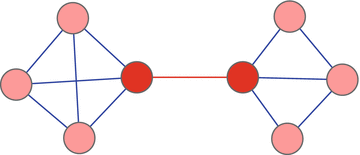
\includegraphics[width=0.65\textwidth]{figures/gn/eb.png}}
}

\frame{
	\frametitle{Edge Betweenness}

	\begin{itemize}
		\item \ccb{$d_{s, i}$} is the \ccp{length of the shortest path} between vertex \ccb{$s$} and vertex \ccb{$i$}.
		\item \ccb{$w_{s, i}$} is the \ccp{number of the shortest paths} from vertex \ccb{$s$} to vertex \ccb{$i$}.
		\item \ccb{$b_{s, i}$} is the \ccp{number of the shortest paths} between vertex \ccb{$s$} to any vertex in graph that pass through vertex \ccb{$i$}.
	\end{itemize}\pause

	Edge betweenness \ccb{$\sigma_{i,j}$} of edge \ccb{$(i,j)$}:
	\ccb{
		\begin{equation*}
			\sigma_{i,j} = \sum_{s \in V}\sigma_{s,i,j}
		\end{equation*}
	} where
	\ccb{
		\begin{equation*}
			\sigma_{s,i,j} = \begin{cases}
				\frac{w_{s,j}}{w_{s,i}}b_{s,i} & d_{s,i} > d_{s,j} \\
				\frac{w_{s,i}}{w_{s,j}}b_{s,j} & d_{s,i} < d_{s,j} \\
				0                              & d_{s,i} = d_{s,j}
			\end{cases}
		\end{equation*}
	}
}

\frame{
	\frametitle{Breath First Search}

	\begin{exampleblock}{}
		\begin{algorithm}[H]
			\SetKwData{x}{x}\SetKwData{y}{y}\SetKwData{z}{z}
			\SetKwFunction{CS}{\sc Breath-First-Search}\SetKwFunction{Return}{\sc Return}\SetKwFunction{Init}{\sc Initialize}
			\SetKwFunction{Up}{\sc Update}\SetKwFunction{Au}{\sc Augment}
			\SetKwInOut{Input}{input}\SetKwInOut{Output}{output}
			\CS{$G=(V,E), s$}
			\BlankLine
			$d_{s,s} \leftarrow 0, w_{s,s} \leftarrow 1, b_{s,s} \leftarrow 0$,
			$Q \leftarrow \{s\}, L \leftarrow \{s\}$\;
			\For{each vertex $v \in V - \{s\}$}{
				$d_{s,v} \leftarrow \infty, w_{s,v} \leftarrow 0, b_{s,v} \leftarrow 1$\;
			}
			\While{$Q$ is not empty}{
			Dequeue $i \leftarrow Q$\;
			\For{each vertex $j$ where $(i,j) \in E$}{
			\If{$d_{s,j} \neq \infty$ and $d_{s,j} = d_{s,i}+1$}{
			$w_{s,j} = w_{s,j}+w_{s,i}$\;
			}
			\If{$d_{s,j}=\infty$}{
				$d_{s,j} = d_{s,i}+1, w_{s,j} = w_{s,i}$, Enqueue $j \rightarrow Q$, Push $j \rightarrow L$\;
			}
			}
			}
			\Return $(d,w,s,L)$\;
		\end{algorithm}
	\end{exampleblock}
}

\frame{
	\frametitle{Reverse Breath First Search}

	\begin{exampleblock}{}
		\begin{algorithm}[H]
			\SetKwData{x}{x}\SetKwData{y}{y}\SetKwData{z}{z}
			\SetKwFunction{CS}{\sc Reverse-Breath-First-Search}\SetKwFunction{Return}{\sc Return}\SetKwFunction{Init}{\sc Initialize}
			\SetKwFunction{Up}{\sc Update}\SetKwFunction{Au}{\sc Augment}
			\SetKwInOut{Input}{input}\SetKwInOut{Output}{output}
			\CS{$G=(V,E),s,w,d,L$}
			\BlankLine
			\While{$L$ is not empty}{
			Pop $i \leftarrow L$\;
			\For{each vertex $j$ where $(i,j) \in E$}{
			\If{$d_{s,i} < d_{s,i}$}{
				$b_{s,i} = 1+\sum_{j}\sigma_{s,i,j}$\;
			}
			\If{$d_{s,i} > d_{s,j}$}{
			$\sigma_{s,i,j} = \frac{w_{s,j}}{w_{s,i}}b_{s,i}$\;
			}
			}
			}
			\Return $\sigma$\;
		\end{algorithm}
	\end{exampleblock}
}

\frame{
	\frametitle{Girvan-Newman Algorithm}

	\begin{exampleblock}{}
		\begin{algorithm}[H]
			\SetKwData{x}{x}\SetKwData{y}{y}\SetKwData{z}{z}
			\SetKwFunction{CS}{\sc Girvan-Newman}\SetKwFunction{Return}{\sc Return}\SetKwFunction{Init}{\sc Initialize}
			\SetKwFunction{Up}{\sc Update}\SetKwFunction{Au}{\sc Augment}
			\SetKwInOut{Input}{input}\SetKwInOut{Output}{output}
			\CS{$G=(V,E)$}
			\BlankLine
			Calculate edge betweenness for each edge in the graph\;
			\While{$E$ is not empty}{
				Let $e$ be the edge with highest edge betweenness\;
				$E \leftarrow E - \{e\}$\;
				Calculate edge betweenness for remaining edges\;
			}
		\end{algorithm}
	\end{exampleblock}
}

\frame{
	\frametitle{Review of Modularity}
	\begin{definition}
		\ccp{Modularity} of a network is a scalar ranging from \ccb{$-\frac{1}{2}$} to \ccb{$1$} that evaluates the density of links inside communities as compared to links between communities.
		\ccb{
			\begin{equation*}
				Q = \frac{1}{4m}\sum_{i \in V, j \in V, c_i = c_j}[A_{ij} - \frac{k_{i}k_{j}}{2m}]
			\end{equation*}
		}
	\end{definition}

	\begin{itemize}
		\item \ccb{$A_{ij}$} is the weight of the edge between \ccb{$i$} and \ccb{$j$}.
		\item \ccb{$k_{i} = \sum_{(i, j) \in E}A_{ij}$} is the sum of the weights of all the edges attached to vertex \ccb{$i$}.
		\item \ccb{$m = \frac{1}{2}\sum_{ij}A_{ij}$},
		\item \ccb{$c_{i}$} is the community of vertex \ccb{$i$}.
	\end{itemize}

	\bigskip
}

\frame{
	\frametitle{Girvan-Newman Algorithm}

	\begin{itemize}
		\item Girvan-Newman algorithm computes the modularity of current community partition, and determined to terminate when the modularity of the resulting partition reaches a \ccp{maximum}.
		\item In complex networks it is often the case that more edges have the \ccp{same highest} edge betweenness. We can remove these edges \ccp{together} to effectively reduce the number of iteration.
	\end{itemize}

	\bigskip
}

\frame{
	\frametitle{Girvan-Newman Algorithm with Modularity}

	\begin{exampleblock}{}
		\begin{algorithm}[H]
			\SetKwData{x}{x}\SetKwData{y}{y}\SetKwData{z}{z}
			\SetKwFunction{CS}{\sc Modularity-Girvan-Newman}\SetKwFunction{Return}{\sc Return}\SetKwFunction{Init}{\sc Initialize}
			\SetKwFunction{Up}{\sc Update}\SetKwFunction{Au}{\sc Augment}
			\SetKwInOut{Input}{input}\SetKwInOut{Output}{output}
			\CS{$G=(V,E)$}
			\BlankLine
			Calculate edge betweenness for each edge in the graph\;
			Calculate modularity $Q$\;
			\While{$E$ is not empty}{
				Let $E'$ be the set of all edges with the highest edge betweenness\;
				Calculate modularity $Q'$ of $G=(V, E - E')$\;
				\If{$Q' < Q$}{
					Break\;
				}
				$E \leftarrow E - E'$\;
				Calculate edge betweenness for remaining edges\;
			}
			\Return{(V, E)}\;
		\end{algorithm}
	\end{exampleblock}

	\bigskip
}

\frame{
	\frametitle{Example}
	Let's start with a simple network.
	\bigskip
	\centerline{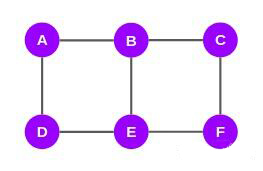
\includegraphics[width=0.45\textwidth]{figures/gn/e0.jpg}}
}

\frame{
	\frametitle{Example}
	Start from vertex \ccb{$A$} and BFS the network to get the shortest paths.
	\bigskip
	\centerline{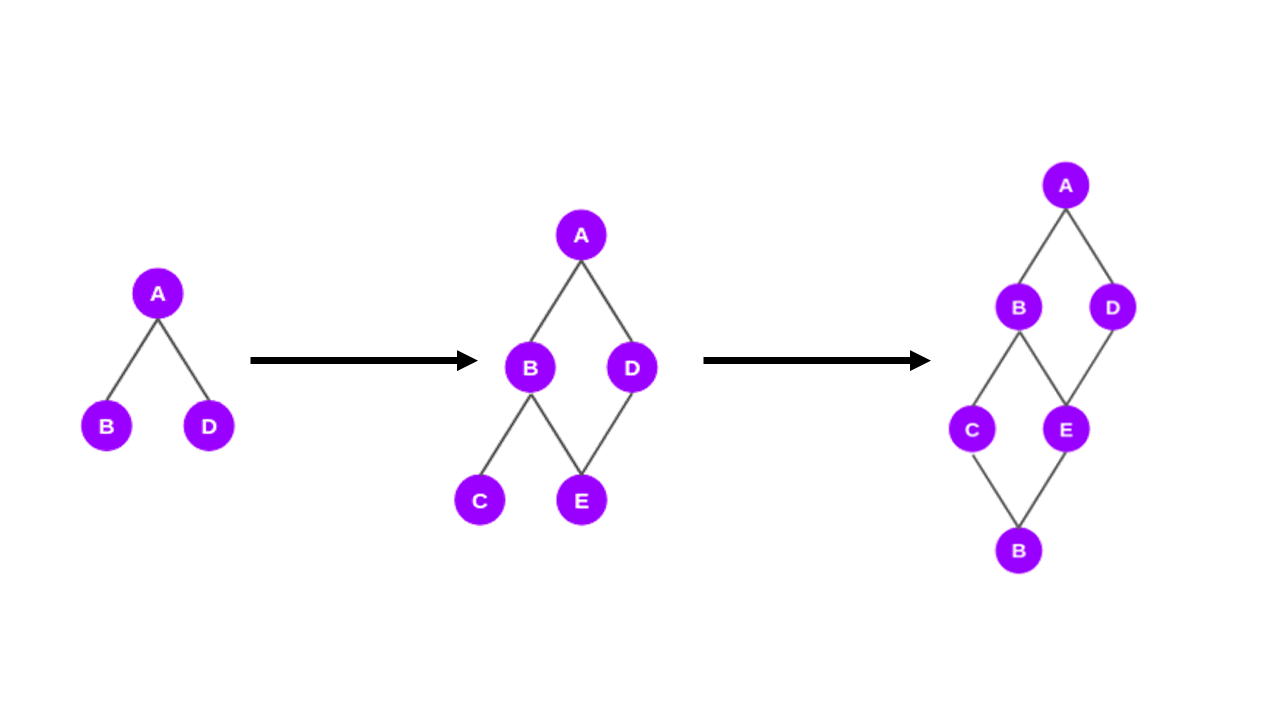
\includegraphics[width=1.1\textwidth]{figures/gn/e1_3.png}}
}

\frame{
	\frametitle{Example}
	Calculate the \ccp{number of the shortest paths} from vertex \ccb{$A$} that pass through vertex \ccb{$u$}.
	\bigskip
	\centerline{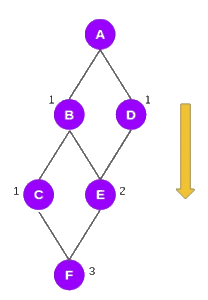
\includegraphics[width=0.35\textwidth]{figures/gn/e4.jpg}}
}

\frame{
	\frametitle{Example}
	Reverse BFS to calculate the \ccp{number of the shortest paths} from vertex \ccb{$A$} that pass through edge \ccb{$e$}.
	\bigskip
	\centerline{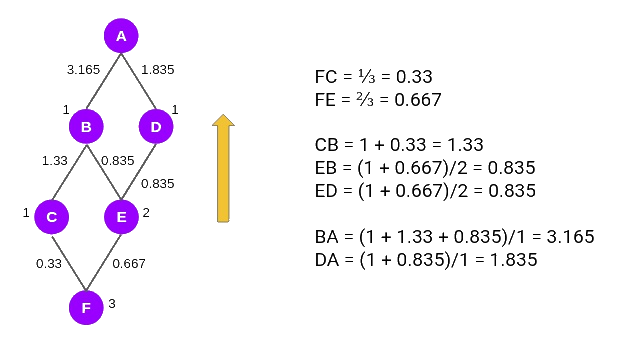
\includegraphics[width=0.85\textwidth]{figures/gn/e5.jpg}}
}

\frame{
	\frametitle{Example}
	Reverse BFS to calculate the \ccp{number of the shortest paths} from vertex \ccb{$A$} that pass through edge \ccb{$e$}.

	\bigskip

	\centerline{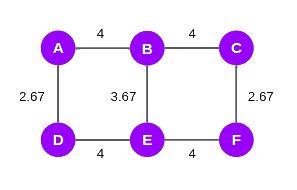
\includegraphics[width=0.55\textwidth]{figures/gn/e6.jpg}}
}

\frame{
	\frametitle{Example}
	Repeat for each vertex and sum them up.

	\bigskip

	\centerline{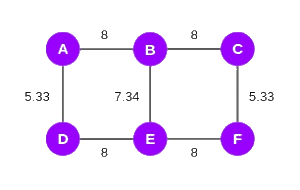
\includegraphics[width=0.55\textwidth]{figures/gn/e7.jpg}}
}

\frame{
	\frametitle{Example}
	Remove all edges with the highest edge betweenness.
	\bigskip
	\centerline{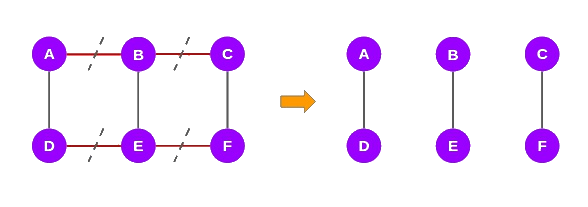
\includegraphics[width=1\textwidth]{figures/gn/e8.jpg}}

	And then we can get three communities.
}

\section{Louvain Algorithm}

\frame{
	\frametitle{Louvain Algorithm}
	\begin{itemize}
		\item Louvain is a multistep technique based on a \ccp{local optimization} of Newman-Girvan modularity in the neighborhood of each node.
		\item After a partition is identified in this way, communities are replaced by \ccp{supernodes}, yielding a smaller weighted network.
		\item The procedure is then iterated, until modularity does not increase any further.
	\end{itemize}\pause
	\centerline{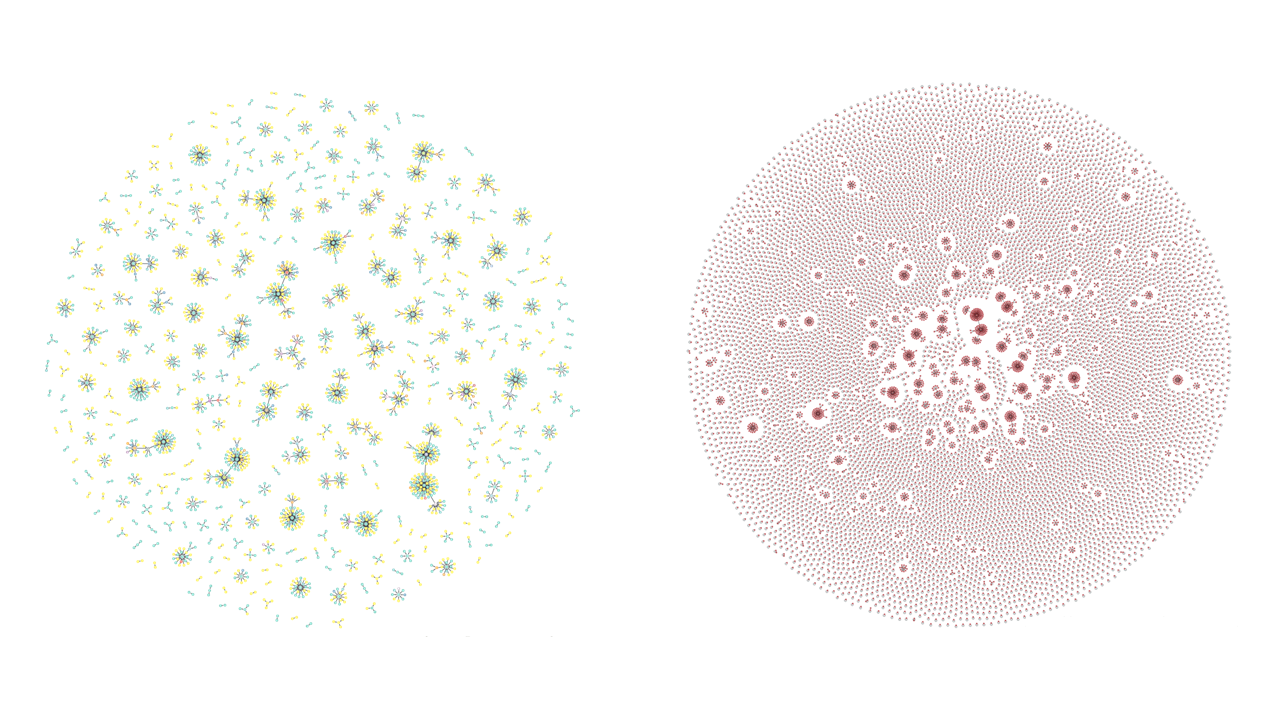
\includegraphics[width=0.9\textwidth]{figures/louvain/v0.png}}
}

\frame{
	\frametitle{Modularity Increment}
	\begin{definition}
		\ccp{Modularity increment} \ccb{$\Delta{Q}$} of \ccb{$(i,j)$} is the \ccp{change of modularity} when removing vertex \ccb{$i$} from its community and then placing it to the community of its neighbor \ccb{$j$}.
	\end{definition}
	\pause
	This removing-placing action can be decomposed into two similar actions:
	\begin{itemize}
		\item [1)] making vertex \ccb{$u$} isolated
		\item [2)] moving the isolated vertex into a community
	\end{itemize}
	\ccb{$\Delta{Q}$} is the sum of \ccb{$\Delta{Q}'$} of these two actions. These two \ccb{$\Delta{Q}'$} can be computed in the same way, for 1) is just the inverse action of 2).
}

\frame{
	\frametitle{Modularity Increment}
	\ccb{
		\begin{equation*}
			\Delta{Q}' = \bigg[\frac{\sum_{in} + k_{i, in}}{2m} - \bigg(\frac{\sum_{tot} + k_{i}}{2m}\bigg)^{2}\bigg] - \bigg[\frac{\sum_{in}}{2m} - \bigg(\frac{\sum_{tot}}{2m}\bigg)^{2} - \bigg(\frac{k_{i}}{2m}\bigg)^{2}\bigg]
		\end{equation*}
	}
	where
	\ccb{
		\begin{itemize}
			\item $\sum_{in}$ is the sum of the weights of the internal edges of $c_{j}$
			\item $\sum_{tot}$ is the sum of the weights of the links incident to vertices in community $c_{j}$
			\item $k_{i, in}$ is the sum of the weights of the links from $i$ to vertices in community $c_{j}$
		\end{itemize}
	}
}

\frame{
	\frametitle{Louvain Algorithm}
	Each iteration, also named \ccp{pass} in Louvain, has two phases.
	\begin{itemize}
		\item [1)] Modularity Optimization
		\item [2)] Community Aggregation
	\end{itemize}

	\centerline{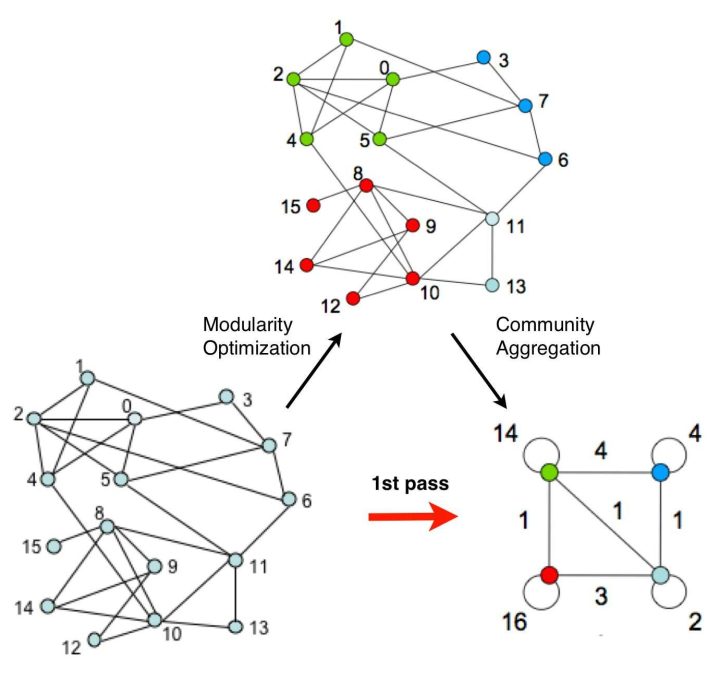
\includegraphics[width=0.65\textwidth]{figures/louvain/2phase.png}}
}

\frame{
	\frametitle{Modularity Optimization}
	\begin{exampleblock}{}
		\begin{algorithm}[H]
			\SetKwData{x}{x}\SetKwData{y}{y}\SetKwData{z}{z}
			\SetKwFunction{CS}{\sc Modularity-Optimization}\SetKwFunction{Return}{\sc Return}\SetKwFunction{Init}{\sc Initialize}
			\SetKwFunction{Up}{\sc Update}\SetKwFunction{Au}{\sc Augment}
			\SetKwInOut{Input}{input}\SetKwInOut{Output}{output}
			\CS{$G=(V,E)$}
			\BlankLine
			\ForEach{$u \in V$}{
				Let $v$ be the neighbor who has the largest modularity increment\;
				\If{this increment is positive}{
					$c_{u} \leftarrow c_{}$
				}
			}
			\Return{c}
		\end{algorithm}
	\end{exampleblock}
}

\frame{
	\frametitle{Example}
	Here is the visualization of phase 1.
	\bigskip
	\centerline{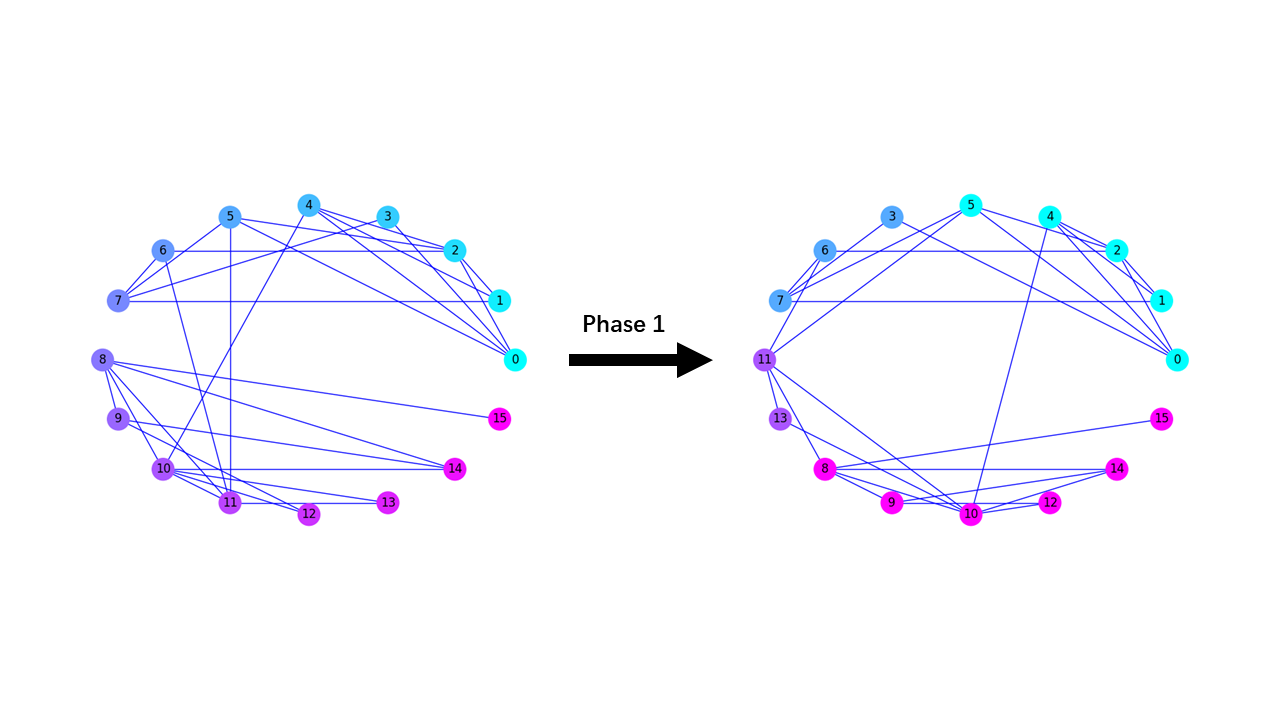
\includegraphics[width=1\textwidth]{figures/louvain/phase1.png}}
}

\frame{
	\frametitle{Community Aggregation}
	\begin{exampleblock}{}
		\begin{algorithm}[H]
			\SetKwData{x}{x}\SetKwData{y}{y}\SetKwData{z}{z}
			\SetKwFunction{CS}{\sc Community-Aggregation}\SetKwFunction{Return}{\sc Return}\SetKwFunction{Init}{\sc Initialize}
			\SetKwFunction{Up}{\sc Update}\SetKwFunction{Au}{\sc Augment}
			\SetKwInOut{Input}{input}\SetKwInOut{Output}{output}
			\CS{$G=(V,E),c$}
			\BlankLine
			\ForEach{unmerged vertex $u$}{
				\ForEach{unmerged vertex $v \in V - \{u\}$ and $c_{u} = c_{v}$}{
					Merge vertex $v$ to $u$\;
				}
				Update internal and external weights of edges\;
			}
			\Return{G,c}
		\end{algorithm}
	\end{exampleblock}
}

\frame{
	\frametitle{Example}
	Here is the visualization of phase 2.
	\begin{itemize}
		\item The weights of edges between two new vertices are determined by sum of the weights of the edges between vertices in the corresponding two communities.
		\item The internal edges of a community leads to a self-loop for the corresponding vertex in the new network.
	\end{itemize}
	\centerline{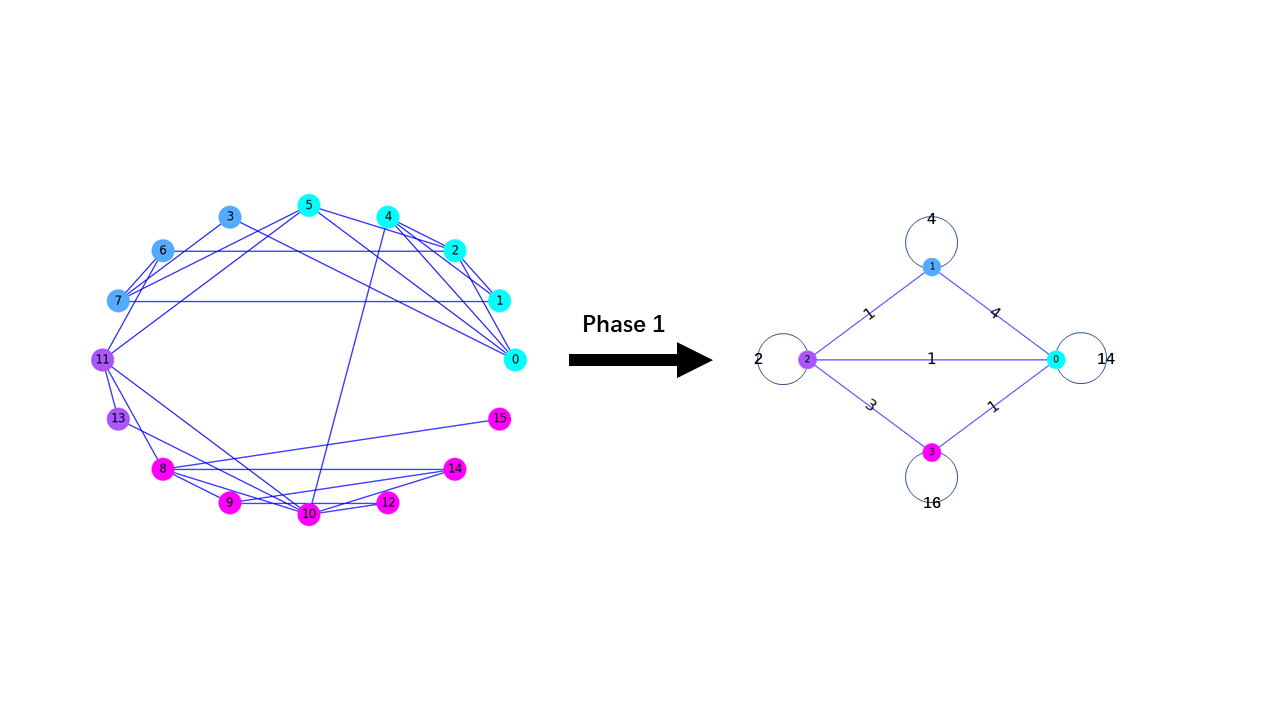
\includegraphics[width=1\textwidth]{figures/louvain/phase2.png}}
}

 \frame{
	\frametitle{Visualization of Louvain Algorithm}
	
	% \centerline{\includemovie{1cm}{1cm}{figures/karoake_louvain.gif}}
	% \animategraphics[width=10cm,height=10cm, autoplay, loop, controls]{24}{figures/louvain/louvain-}
 	\centerline{\animategraphics[width=12cm,height=6cm,autoplay,loop,controls]{36}{figures/louvain_gif/louvain-}{0}{620}}
 }

\section{Parallelization of Louvain Algorithm}


\frame{
	\frametitle{Parallelization of Louvain Algorithm}
	\begin{itemize}
		\item In the original \ccp{serial} algorithm, each vertex examines the communities of its neighbors and makes a choice to chooses a new community based on a function to maximize the calculated change in modularity.
		\item In the \ccp{distributed} and \ccp{parallel} version, all vertices make this choice simultaneously rather than in serial order, updating the graph state after each change.
	\end{itemize}
	\vspace{5mm}
	\centerline{
\includegraphics[width=0.4\textwidth]{figures/louvain/spark.jpeg}}
	
}

\frame{
	\frametitle{Parallelization of Louvain Algorithm}
	\begin{exampleblock}{}
		\begin{algorithm}[H]
			\SetKwData{x}{x}\SetKwData{y}{y}\SetKwData{z}{z}
			\SetKwFunction{CS}{\sc Parallel-Louvain}\SetKwFunction{Return}{\sc Return}\SetKwFunction{Init}{\sc Initialize}
			\SetKwFunction{Up}{\sc Update}\SetKwFunction{Au}{\sc Augment}
			\SetKwInOut{Input}{input}\SetKwInOut{Output}{output}
			\CS{$G=(V,E)$}
			\BlankLine
			\While{True}{
				\ForEach{vertex $u \in V$}{
					Modularity Optimization on vertex $u$ in parallel to get modularity increment $\Delta{Q}_{u}$\;
				}
				$\Delta{Q} \leftarrow \sum_{u \in V}\Delta{Q}_{u}$\;
				\If{$\Delta{Q} \le 0$}{
					Break\;
				}
				Community-Aggregation(G,c)\;
			}
		\end{algorithm}
	\end{exampleblock}
}

\frame{
	\frametitle{Parallelization of Louvain Algorithm}
	The flowchart of the parallel Louvain algorithm:
	\centerline{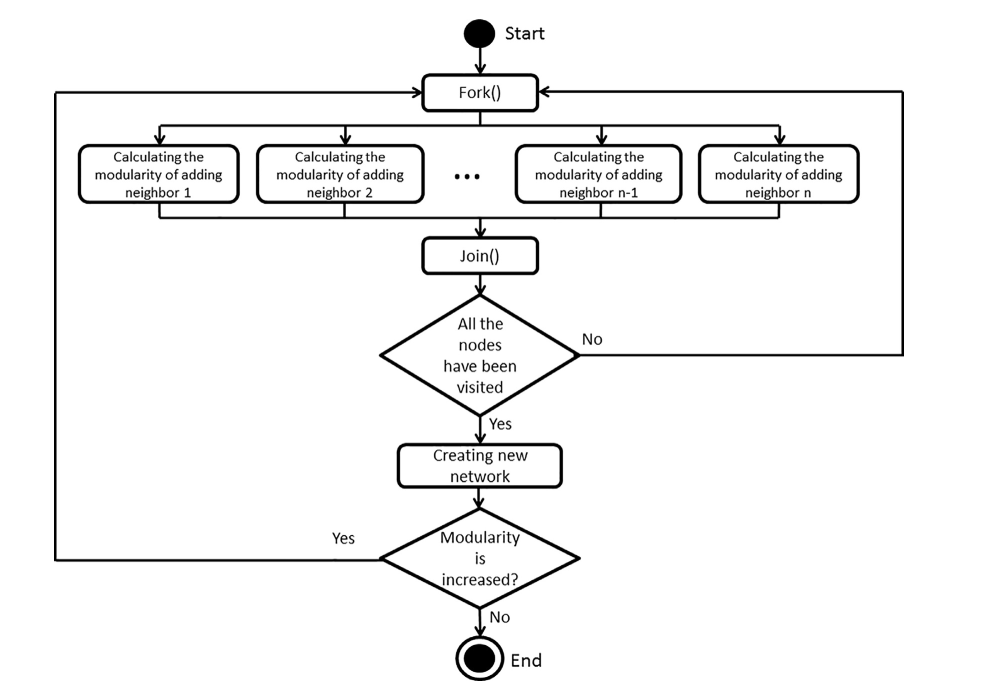
\includegraphics[width=1\textwidth]{figures/louvain/p_flowchart.jpg}}
}

\frame{
	\frametitle{Parallelization of Louvain Algorithm}
	Practically, It is a good choice to implement a parallel algorithm on \ccp{Spark}, which is a cluster computing framework supporting reusing a working set of data across multiple parallel operations while retaining the scalability and fault tolerance of \ccp{MapReduce}.

	To describe the algorithm using MapReduce framework:
	\begin{itemize}
		\item [1)] Get information of adjacent vertices.
		      \begin{itemize}
			      \item [a)] Map: produce information of adjacent vertices \ccb{$\text{VertexData}$};
			      \item [b)] Reduce: get information of adjacent vertices \ccb{$(\text{Id}, \text{Array}[\text{VertexData}])$}.
		      \end{itemize}
		\item [2)] Get the new community \ccb{$(\text{Id}, \text{getBestCommunity}(\text{Array}[\text{VertexData}]))$}
		\item [3)] Update the information in the network and merge vertices to go to next iteration.
	\end{itemize}
}

\section{Improvement of Louvain Algorithm}

\frame{
	\frametitle{Drawbacks of Louvain Algorithm}
	In the Louvain algorithm, a node may be moved to a different community, while it may have acted as a "bridge" between different communities. Removing such a node disconnects the nodes in the old community.
	
	\vspace{5mm}
	
	\centerline{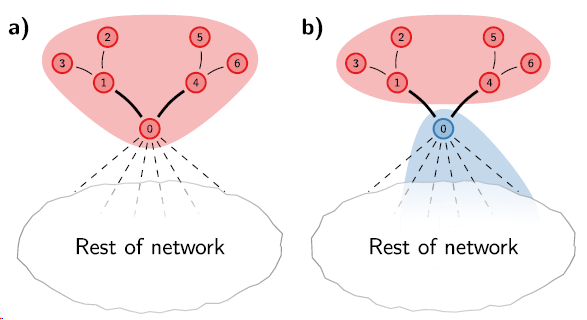
\includegraphics[width=0.8\textwidth]{figures/louvain/louvain_drawback.png}}
}

\frame{
	\frametitle{Leiden Algorithm}
	The Leiden algorithm is more complex than the Louvain algorithm. It consists of three phases:
	\begin{itemize}
		\item [1)] Local moving of nodes.
		\item [2)] Refinement of the partition.
		\item [3)] Aggregation of the network based on the refined partition, use the non-refined partition to create an initial partition for the aggregate network.
	\end{itemize}
}

\frame{
	\frametitle{Leiden Algorithm}

	\centerline{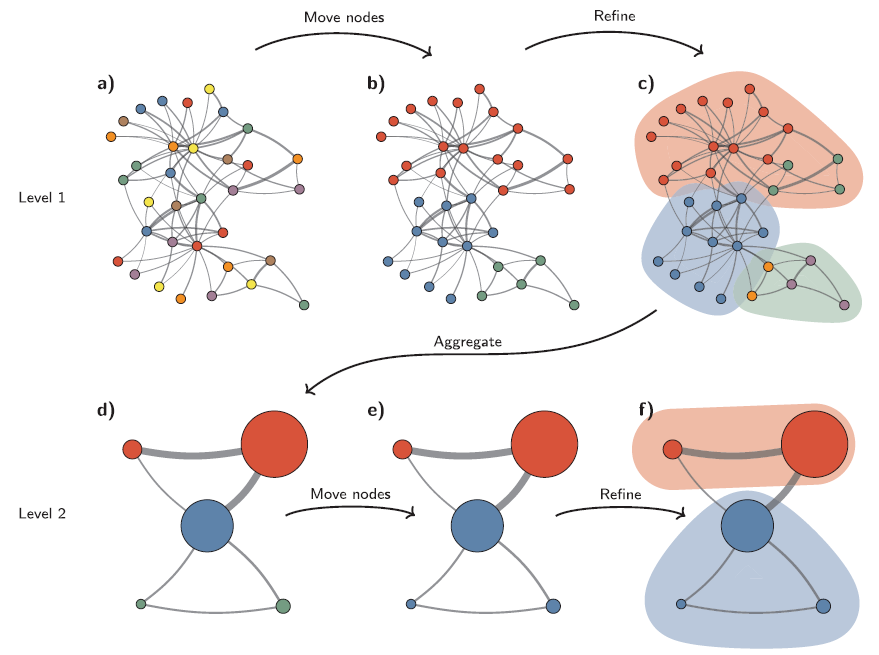
\includegraphics[width=0.5\textwidth]{figures/louvain/leiden.png}}

	\begin{itemize}
		\item The Leiden algorithm starts from a singleton partition (\ccb{$a$}).
		\item The algorithm moves individual nodes from one community to another to find a partition (\ccb{$b$}), which is then refined (\ccb{$c$}).
		\item An aggregate network (\ccb{$d$}) is created based on the refined partition, using the non-refined partition to create an initial partition for the aggregate network.
	\end{itemize}
}

\frame{
	\frametitle{Leiden Algorithm}

	\centerline{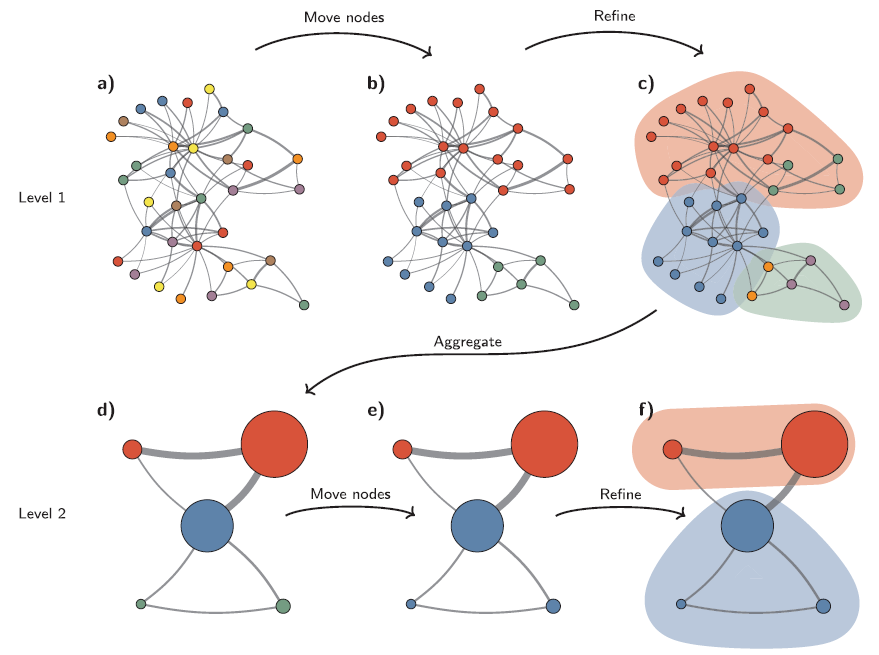
\includegraphics[width=0.5\textwidth]{figures/louvain/leiden.png}}

	\begin{itemize}
		\item The algorithm then moves individual nodes in the aggregate network (\ccb{$e$}).
		\item In this case, refinement does not change the partition (\ccb{$f$}).
		\item These steps are repeated until no further improvements can be made.
	\end{itemize}
}

\frame{
	\frametitle{Comparison Between Louvain and Leiden}

	\centerline{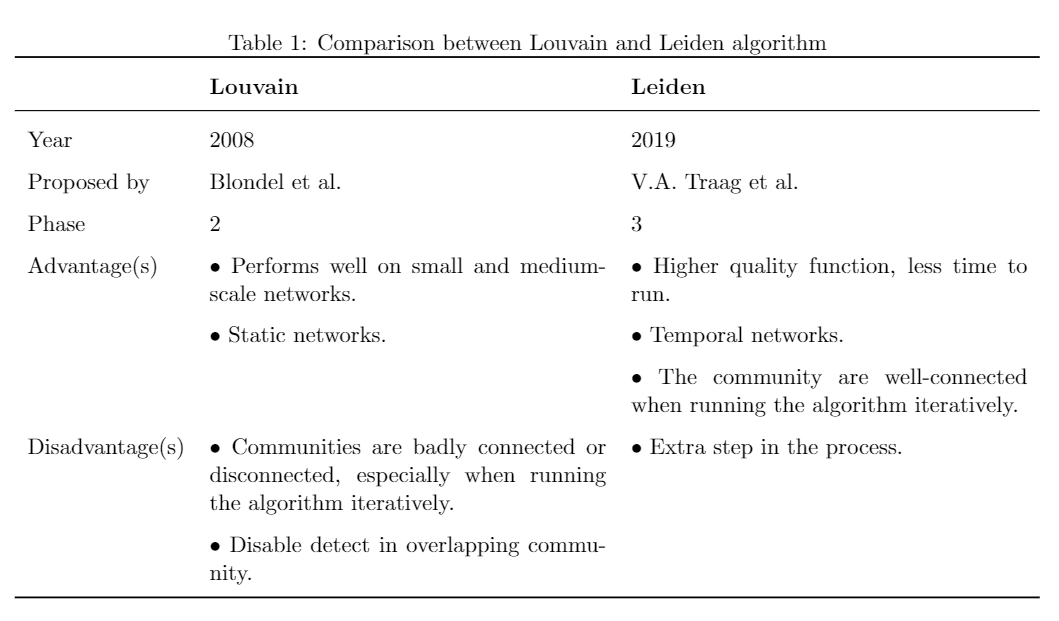
\includegraphics[width=1.05\textwidth]{figures/louvain/compare.jpg}}
}

\section{Applications of Community Detection}

\frame{
	\frametitle{Applications in social networks}
	An social network is the interaction of people with each other through the web. Community detection has been widely used in this area.

	Various studies have utilized different community detection methods to analyze public emotional reaction and visualize relationships and characteristics.
	\centerline{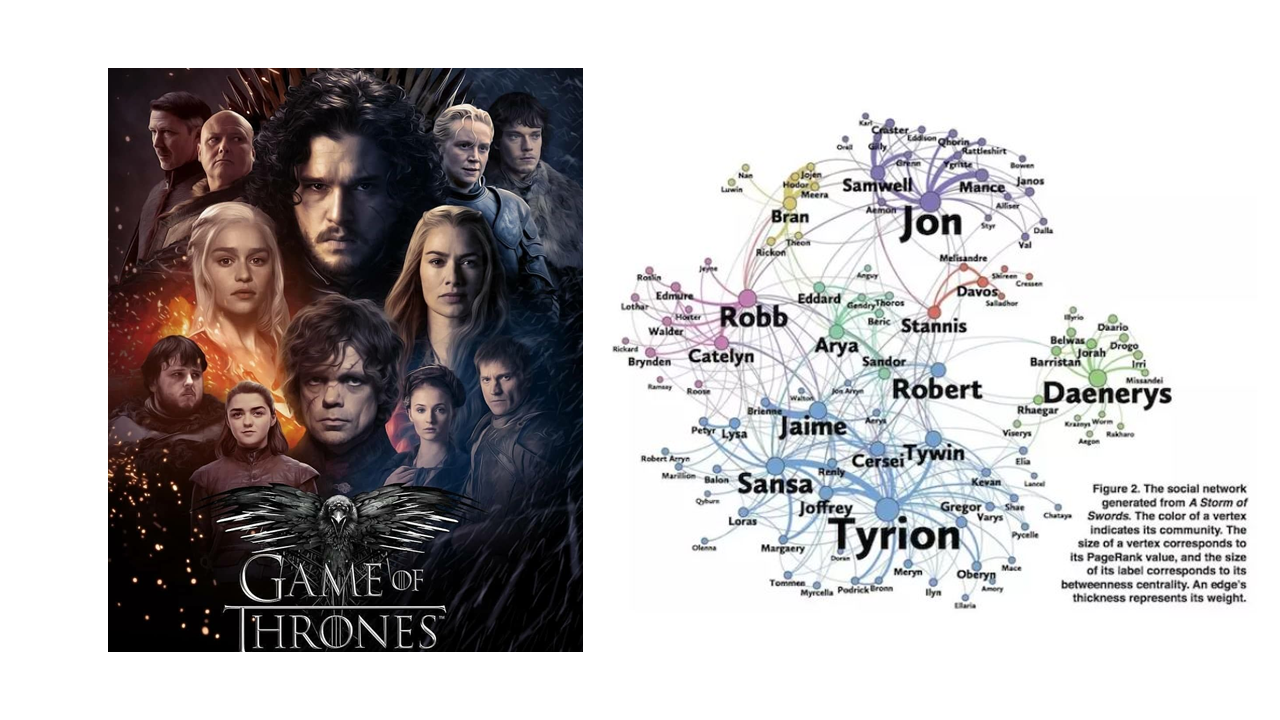
\includegraphics[width=1\textwidth]{figures/app/combine.png}}
}

\frame{
	\frametitle{Applications in biological networks}
	Researchers have proposed an algorithm called \ccp{disease-gene network detecting algorithm}, based on Principal Component Analysis (PCA), which can extract the communities in a diseasome bipartite network.

	This algorithm is aimed at disease prevention and medical diagnosis.
	\centerline{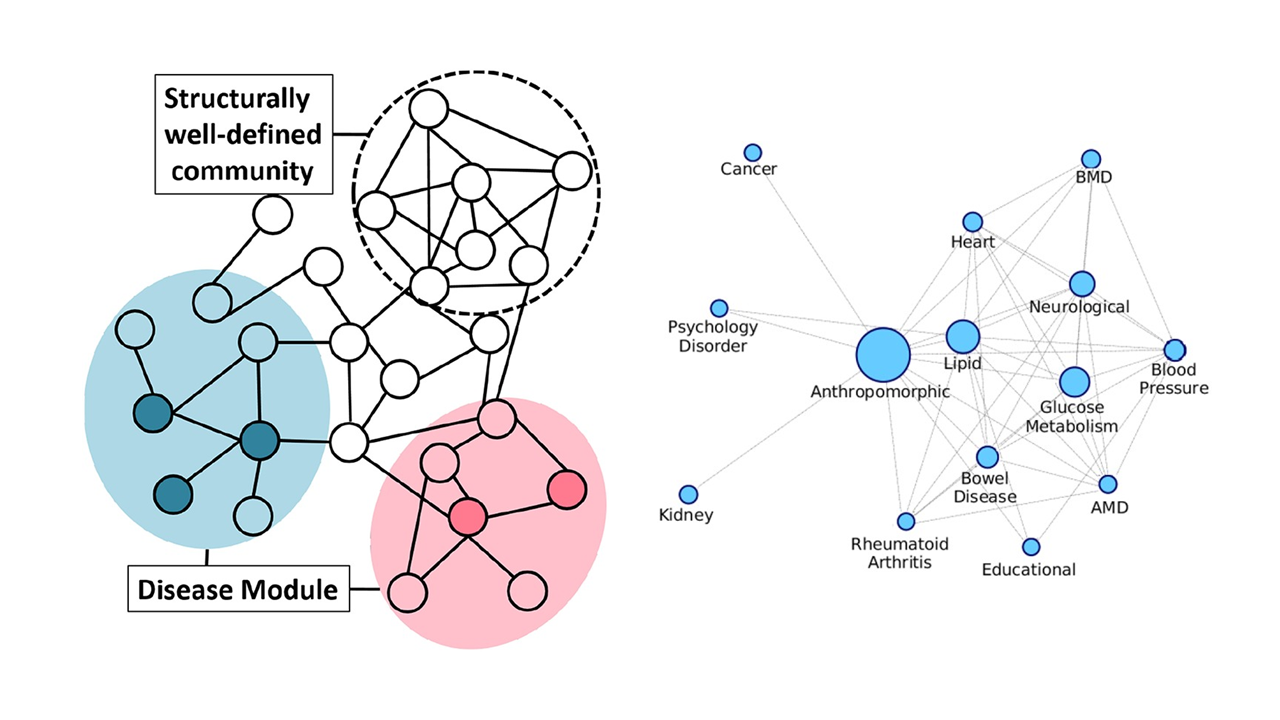
\includegraphics[width=0.9\textwidth]{figures/app/bio.png}}
}

\frame{
	\frametitle{Applications in economics}
	In the \ccp{stock market}, each stock can be represented by a vertex and edge represents the correlations of stock values in the market. Researchers have stated the way to construct the network of stock market and detect communities in it.
	They revealed community structure by using modularity \ccb{$Q$}, which helps to the analysis and decision-making of the stock market.
	
	\begin{figure}
	\centerline{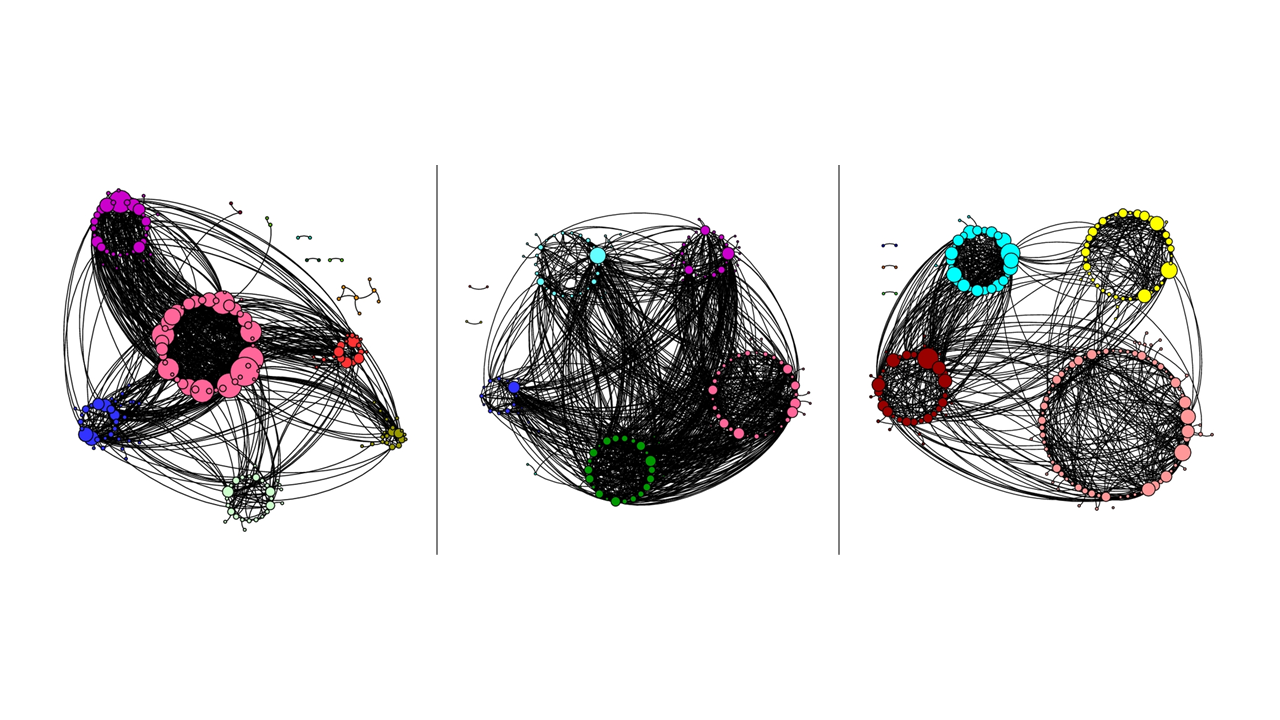
\includegraphics[width=0.75\textwidth]{figures/app/stock.png}}
	\caption{Several pictures of stock networks. Different node colors represent different communities and node sizes reflect its degree.}
	\end{figure}

}

\section{Conclusion}

\frame{
	\frametitle{Future Direction}
	\ccp{Deep learning} --- a promising direction of community detection. Beyond simply examining network topologies for detecting communities, some strategies also explore semantic descriptions as node features in the data.

	\centerline{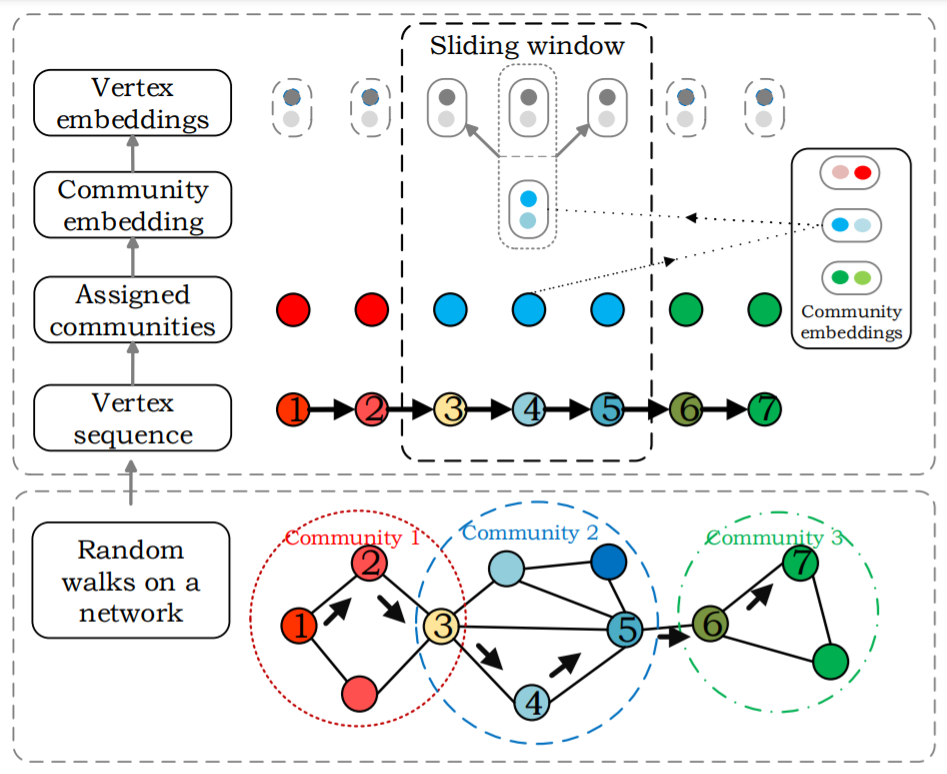
\includegraphics[width=0.65\textwidth]{figures/conc/dl.jpg}}
}

\frame{
	\frametitle{Open problems}
	There are still so many broad challenges in community detection. For example:
	\begin{itemize}
		\item Network \ccp{dynamics}
		\item \ccp{Large-scale} networks
		\item \ccp{Inaccurate} number of communities
	\end{itemize}
}

\frame{
	\frametitle{Network dynamics}
	Changing dynamics can affect either the network topology or the node attributes. Topological changes not only cause changes in a local community, but also leads to devastating changes across an entire network.

	Actually, a lot of methods have been used to deal with sequential data in machine learning, such as \ccp{long short-term memory} (\ccp{LSTM}). Therefore, deep learning methods for detecting communities with dynamic spatial and temporal properties are very likely to be developed.

	\centerline{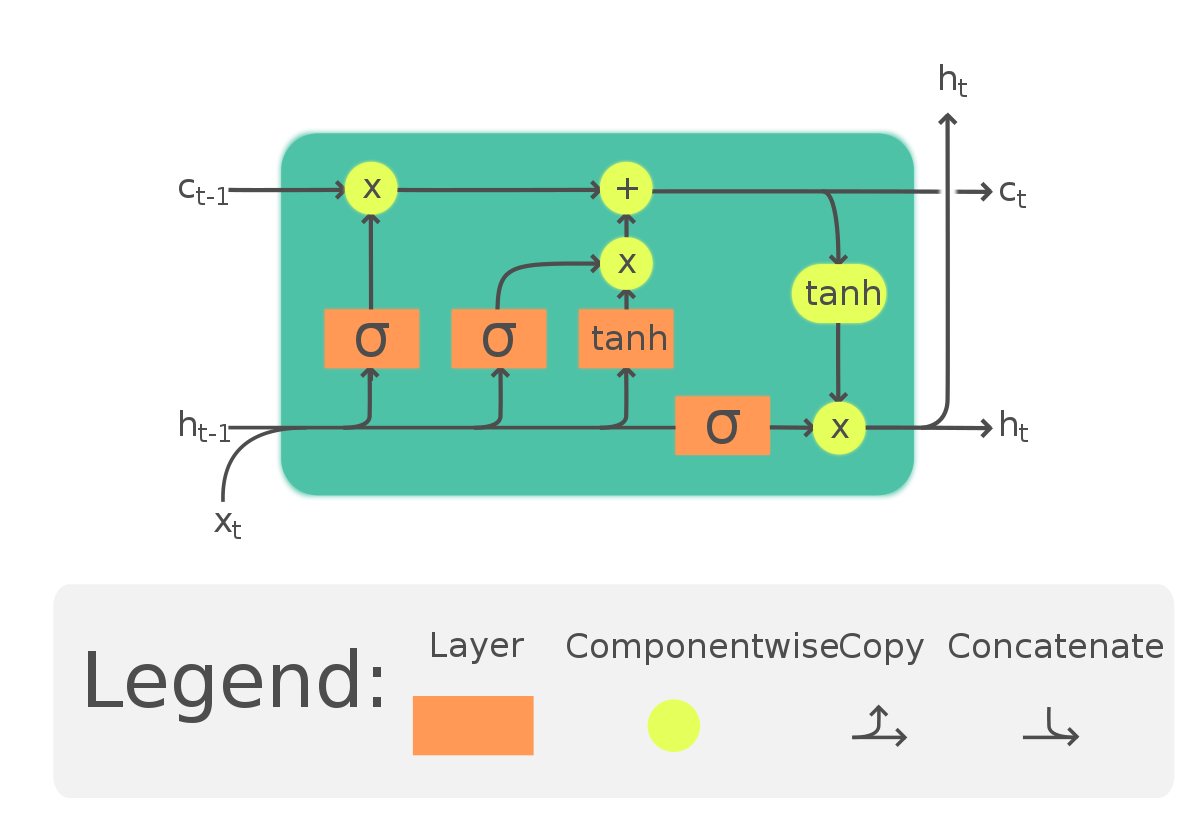
\includegraphics[width=0.6\textwidth]{figures/conc/LSTM.png}}
}

\frame{
	\frametitle{Large-scale networks}
	Nowadays, large-scale networks can contain millions of nodes, edges, and structural patterns, as networks like Twitter and Weibo, which has also brought a lot of problems.

	For instance, large-scale networks may have their inherent characteristics, such as \ccp{scale-free}. There exists lots of mega hubs in the network, which can influence the performance of algorithms in community detection.
	
	\vspace{5mm}
	
	\centerline{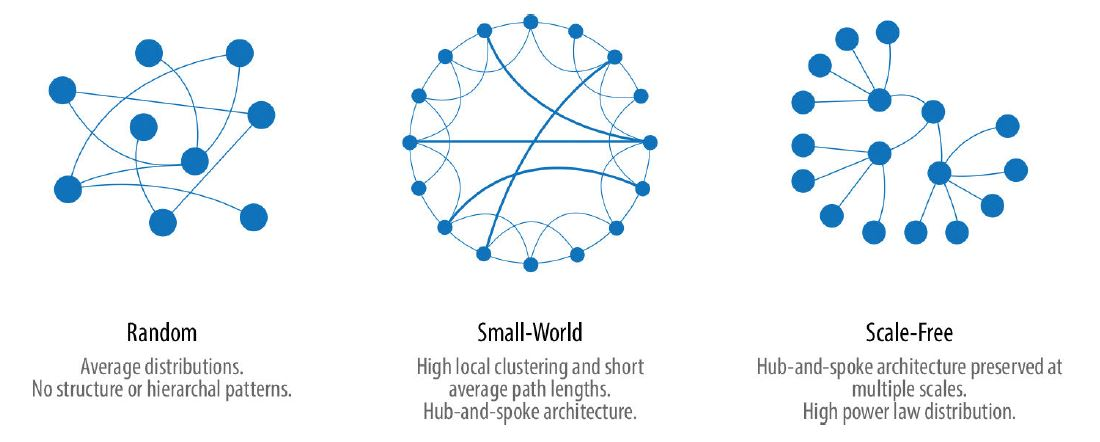
\includegraphics[width=0.75\textwidth]{figures/app/scalefree.jpg}}
	
}

\frame{
	\frametitle{Inaccurate number of communities}
	In fact, most algorithms of the community detection require the \ccp{number of communities} beforehand as a hyperparameter, including deep learning.

	Two common solutions:
	\begin{itemize}
		\item Using \ccp{modularity-based} algorithm, like Girvan-Newman or Louvain
		\item Using \ccp{statistical} interference
	\end{itemize}

	Unfortunately, both methods have poor performance under large-scale networks.
}


\end{document}
